\setcounter{section}{4}
\setcounter{subsection}{12}
\setcounter{subsubsection}{0}

\subsection{Floating Objects\\浮动对象}
\begin{docTcbKey}{floatplacement}{=\meta{values}}{no default, initially \texttt{htb}}
Sets \meta{values} as default values for the usage of \refKeyLe{/tcb/float}
and \refKeyLe{/tcb/float*}.
Feasible are the usual parameters for floating objects.

设置\meta{values}为\refKeyLe{/tcb/float}和\refKeyLe{/tcb/float*}的默认值。可选值是浮动对象的常用参数。
\begin{dispListing}
\tcbset{enhanced,colback=red!5!white,colframe=red!75!black,
watermark color=red!15!white}

\begin{tcolorbox}[floatplacement=t,%浮动框将被放置在页面顶部。
float,%将浮动框放置在浮动环境中,可以让它在页面上自动调整位置。
title=Floating box from |floatplacement|,%浮动框的标题
watermark text={I am floating}]%在浮动框上添加一个水印文本
This floating box is placed at the top of a page.这个浮动框被放置在页面顶部。
\end{tcolorbox}
\end{dispListing}
\end{docTcbKey}
{\tcbusetemp}


\begin{docTcbKey}{float}{\colOpt{=\meta{values}}}{default from \texttt{floatplacement}}
Turns the box to a floating object where \meta{values} are the
usual parameters for such floating objects.
If they are not used, the placement uses the default values given by
|floatplacement|.

将盒子转为浮动对象,\meta{values}是其浮动位置的参数。如果没有指定,那么将使用 |floatplacement| 设置的默认值。
\begin{dispListing}
\begin{tcolorbox}[float, title=Floating box from |float|,
enhanced,watermark text={I'm also floating}]
This box floats to a feasible place automatically. You do not have to
use a numbering for this floating object.

这个盒子会自动浮动到合适的位置上,您不需要为这个浮动对象使用编号。
\end{tcolorbox}
\end{dispListing}
\end{docTcbKey}
{\tcbusetemp}


\begin{docTcbKey}{float*}{\colOpt{=\meta{values}}}{default from \texttt{floatplacement}}
Identical to \refKeyLe{/tcb/float}, but for wide boxes spanning the whole page
width of two column documents or in conjunction with the packages
|multicol| or |paracol|. Note that you have to set |width=\textwidth|
additionally, if the box should span the whole page width in these cases!

与 \refKeyLe{/tcb/float} 相同,但适用于跨越双栏文档整个页面宽度或与 |multicol| 或 |paracol| 包结合使用的宽框。请注意,在这些情况下,如果框应跨越整个页面宽度,则必须另外设置 |width=\textwidth|!

% 同\refKeyLe{/tcb/float}一样,但用在|multicol|或|paracol|的双栏中排版横跨页面的盒子。 
% 注意,你需要额外设置 |width=\textwidth|, 如果需要让盒子在这些情况下横跨页面的话!
\begin{dispListing}
\begin{tcolorbox}[float*=b, title=Floating box from |float*|,width=\textwidth,
enhanced,watermark text={I'm also floating}]
In this single column document, you will see no difference to |float|.
\end{tcolorbox}
\end{dispListing}
\end{docTcbKey}
{\tcbusetemp}




\begin{docTcbKey}{nofloat}{}{style, initially set}
Turns the floating behavior off.

关闭浮动行为。
\end{docTcbKey}


\begin{docTcbKey}[][doc new=2014-09-19]{every float}{=\meta{code}}{no default, initially empty}
For floating objects, the \refKeyLe{/tcb/before} and \refKeyLe{/tcb/after}
settings are ignored. Instead, the given \meta{code} is inserted before
a floating box. If the box is \refKeyLe{/tcb/breakable}, the given \meta{code} is
inserted before every part of the break sequence.
The most common use case is |every float=\centering|.

对于浮动对象,\refKeyLe{/tcb/before}和\refKeyLe{/tcb/after}设置将被忽略。相反,给定的\meta{code}会在浮动框之前插入。如果框是\refKeyLe{/tcb/breakable},则给定的\meta{code}会在断点序列的每个部分之前插入。最常见的用法是|every float=\centering|。

% 浮动对象会忽略\refKeyLe{/tcb/before}和\refKeyLe{/tcb/after}的设置。
% 取而代之的是, \meta{code}会被插入到浮动盒子之前。
% 如果盒子设置为\refKeyLe{/tcb/breakable}, 那么\meta{code}会被插入每个分开的部分的前部。
% 最常见的用例是|every float=\centering|.

\begin{dispListing}
\tcbox[float=htb,title={Floating box},every float=\centering,
colback=blue!50!black,colframe=blue!50!white,colbacktitle=blue!10!white,
coltitle=black,center title]
{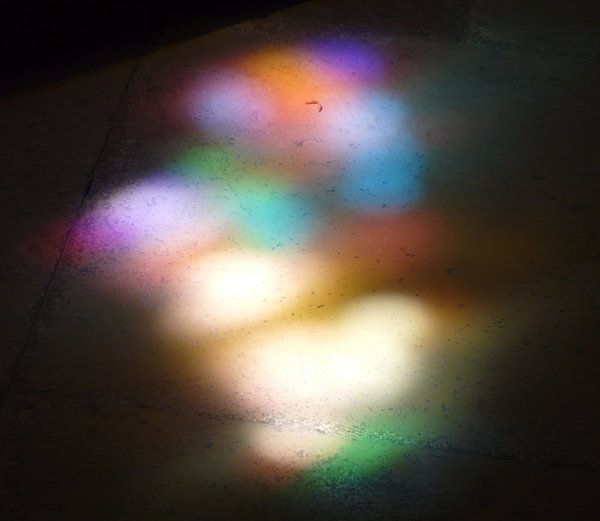
\includegraphics[height=6cm]{lichtspiel.jpg}}
\end{dispListing}
{\tcbset{reset}\tcbusetemp}

\end{docTcbKey}